

Tenemos: 

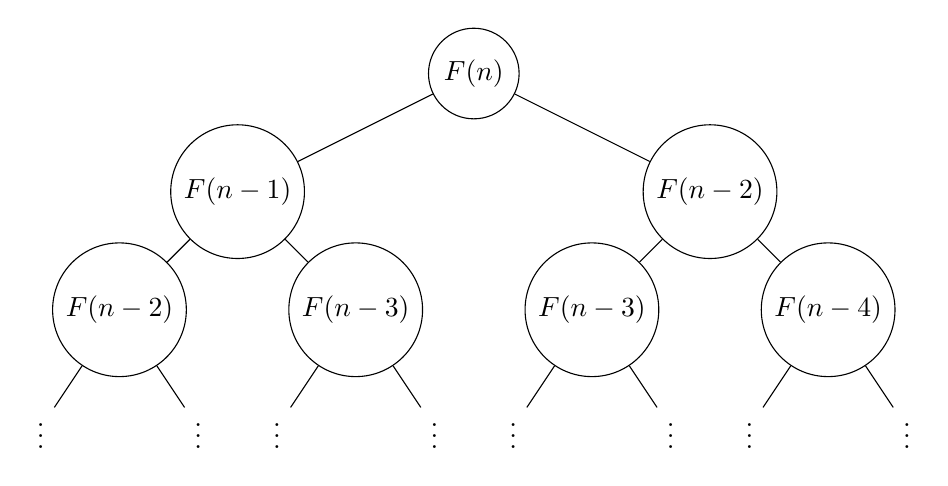
\begin{tikzpicture}[level/.style={sibling distance=60mm/#1}]
    \node [circle,draw] (n1) {$F(n)$}
      child {
        node [circle,draw] (n2) {$F(n-1)$}
          child {
            node [circle,draw] (n4) {$F(n-2)$}
            child {node {$\vdots$}
              edge from parent
            }
            child {node {$\vdots$}
              edge from parent
            }
          }
          child {
            node [circle,draw] (n5) {$F(n-3)$}
            child {node {$\vdots$}
              edge from parent
            }
            child {node {$\vdots$}
              edge from parent
            }
          }
      }
      child {
        node [circle,draw] (n3) {$F(n-2)$}
        child {
          node [circle,draw] (n6) {$F(n-3)$}
          child {node {$\vdots$}
            edge from parent
          }
          child {node {$\vdots$}
            edge from parent
          }
        }
        child {
          node [circle,draw] (n7) {$F(n-4)$}
          child {node {$\vdots$}
            edge from parent
          }
          child {node {$\vdots$}
            edge from parent
          }
        }
      };
    \end{tikzpicture}